% 2006 湖北理科第15题：源图中的莱布尼茨三角形分数排列。
\begin{tikzpicture}[x=0.86cm, y=0.78cm, font=\small]
  \node at (0, 0) {$\dfrac{1}{1}$};

  \node at (-0.5, -1) {$\dfrac{1}{2}$};
  \node at ( 0.5, -1) {$\dfrac{1}{2}$};

  \node at (-1, -2) {$\dfrac{1}{3}$};
  \node at ( 0, -2) {$\dfrac{1}{6}$};
  \node at ( 1, -2) {$\dfrac{1}{3}$};

  \node at (-1.5, -3) {$\dfrac{1}{4}$};
  \node at (-0.5, -3) {$\dfrac{1}{12}$};
  \node at ( 0.5, -3) {$\dfrac{1}{12}$};
  \node at ( 1.5, -3) {$\dfrac{1}{4}$};

  \node at (-2, -4) {$\dfrac{1}{5}$};
  \node at (-1, -4) {$\dfrac{1}{20}$};
  \node at ( 0, -4) {$\dfrac{1}{30}$};
  \node at ( 1, -4) {$\dfrac{1}{20}$};
  \node at ( 2, -4) {$\dfrac{1}{5}$};

  \node at (-2.5, -5) {$\dfrac{1}{6}$};
  \node at (-1.5, -5) {$\dfrac{1}{30}$};
  \node at (-0.5, -5) {$\dfrac{1}{60}$};
  \node at ( 0.5, -5) {$\dfrac{1}{60}$};
  \node at ( 1.5, -5) {$\dfrac{1}{30}$};
  \node at ( 2.5, -5) {$\dfrac{1}{6}$};

  \node at (-3, -6) {$\dfrac{1}{7}$};
  \node at (-2, -6) {$\dfrac{1}{42}$};
  \node at (-1, -6) {$\dfrac{1}{105}$};
  \node at ( 0, -6) {$\dfrac{1}{140}$};
  \node at ( 1, -6) {$\dfrac{1}{105}$};
  \node at ( 2, -6) {$\dfrac{1}{42}$};
  \node at ( 3, -6) {$\dfrac{1}{7}$};

  \node at (0, -7) {$\cdots\cdots$};
\end{tikzpicture}
